% Specify what kind of document this is
\documentclass[10pt, letterpaper]{article}


% Load extra packages to get access to special symbols and commands
\usepackage{fullpage}
\usepackage{color}
\usepackage{amsmath}
\usepackage{amssymb}
\usepackage{graphicx}
\usepackage{subfigure}

% Title information
\title{CS 224W Project}
\author{Nikhil Johri
  \and Zahan Malkani
  \and Ying Wang}
\date{}

% Begin
\begin{document}

\maketitle

\section{Introduction}

\section{Dataset}


\begin{table}[htb]
\centering
\begin{tabular}{|c|c|}
\hline
Users &65,888 \tabularnewline \hline
Reviews &152,327 \tabularnewline \hline
Businesses &9600 \tabularnewline \hline
Reviews per user &Mean = 2.31, Median = 1, STD = 3.83 
\tabularnewline \hline
Reviews per business &Mean = 22.08, Median = 6, STD = 57.4 
\tabularnewline \hline
\end{tabular}
\caption{ Dataset statistics }
\label{stats}
\end{table}


\begin{figure}[htb]
  \centering
  \subfigure[small][Users]
            {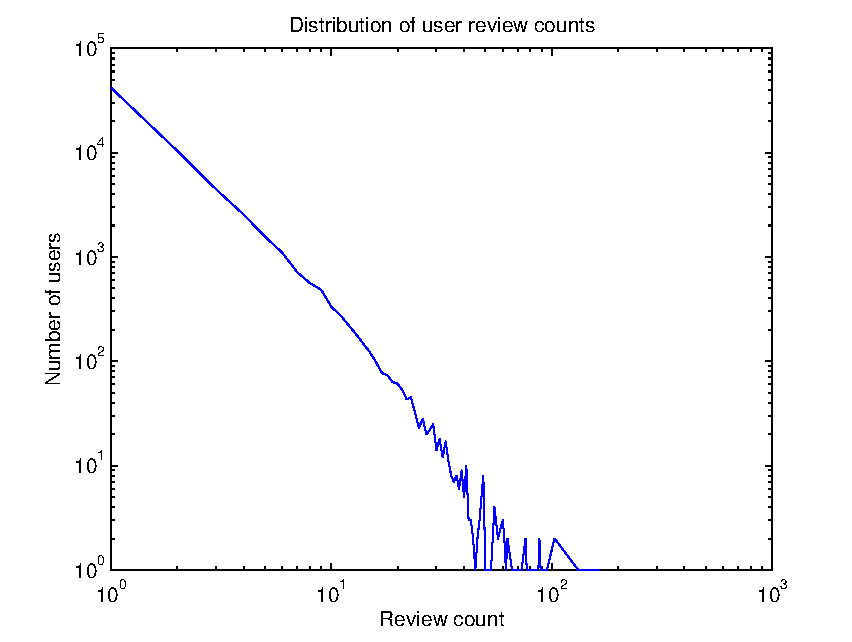
\includegraphics[width = 210pt]{images/u_hist.pdf}}
  \subfigure[small][Businesses]
            {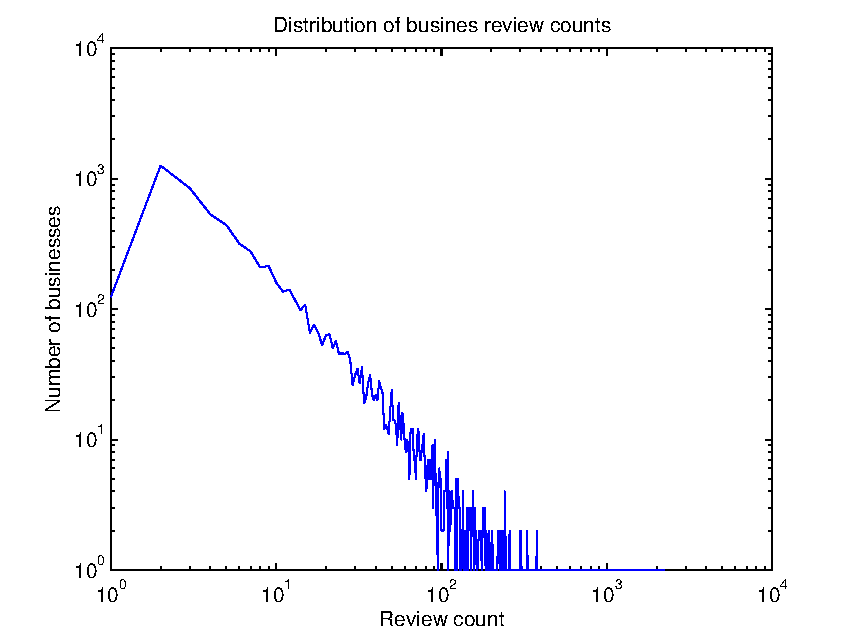
\includegraphics[width = 210pt]{images/b_hist.pdf}}

            \caption{Review count distributions}
            \label{review_count}

\end{figure}

\end{document}
